\chapter{Implementierung}\label{Chap:Implementierung}

\section{Projektplan für den Feasibility Check}
Für die Entwicklung des automatisierten technischen Feasibility Checks wurde zu Beginn ein Projektplan in Form eines GANTT-Diagramms erstellt, der in Abbildung \ref{fig:roadmap} dargestellt ist. Dieser Plan ist in mehrere Swimlanes unterteilt und umfasst die Erarbeitung der Anforderungen, den Entwurf des Datenbankdesigns, die Backend-Entwicklung, die Frontend-Entwicklung sowie das Testen des Systems. Zusätzlich wurden für die Benutzer spezifische Meilensteine definiert, die in der unteren Zeile des Diagramms veranschaulicht werden.

\begin{figure}[!htbp]
    \centering
    \includegraphics[width=1\textwidth]{bilder/Roadmap.pdf}
    \caption{Feasibility Check Projektplan}
    \label{fig:roadmap}
\end{figure}

Die geplanten Maßnahmen für die ersten zwei Monate konnten weitgehend umgesetzt werden, mit Ausnahme der Endanwender-Tests. In den darauffolgenden Monaten lag der Schwerpunkt auf der Überarbeitung bestehender Algorithmen im Backend, da wiederholt neue Ausnahmefälle identifiziert wurden. Auch das Frontend wurde mehrfach angepasst, um den aktuellen Anforderungen gerecht zu werden. Dadurch konnten alle optionale Meilensteine, sowie die Implementierung weiterer Checks inklusive des er \gls{substrate} Checks, nicht realisiert werden – unter anderem aufgrund einer zu optimistischen Zeiteinteilung.

Aktuell sind das Datenbankdesign und das Backend bereits vom Testing-System auf das Staging-System ausgerollt worden und werden dort von einzelnen Anwendern getestet. Für das Backend wurden zudem Unittests entwickelt, was im Frontend leider nicht mehr möglich war. Weitere geplante Meilensteine konnten letztlich aufgrund von Zeitbeschränkungen nicht umgesetzt werden.


\section{Entwicklungsumgebung}
Tools und Technologien, die verwendet wurden (IDE, Frameworks, Datenbank-Tools).
Angular, Visual Studio Code, 
C\#, Visual Studio,
Oracle, Pl sql developer

\section{Implementierung des Feasibility Checks}
Detaillierte Beschreibung des Implementierungsprozesses.
(Beschreibung der C\#-Implementierung, inklusive wichtiger Klassen und Methoden.
flussdiagramme
nhibernate, try catch blöcke,)
\section{Integration}
Wie die verschiedenen Teile (Frontend, Backend, Datenbank) miteinander interagieren.

\begin{figure}[!h]
    \centering
    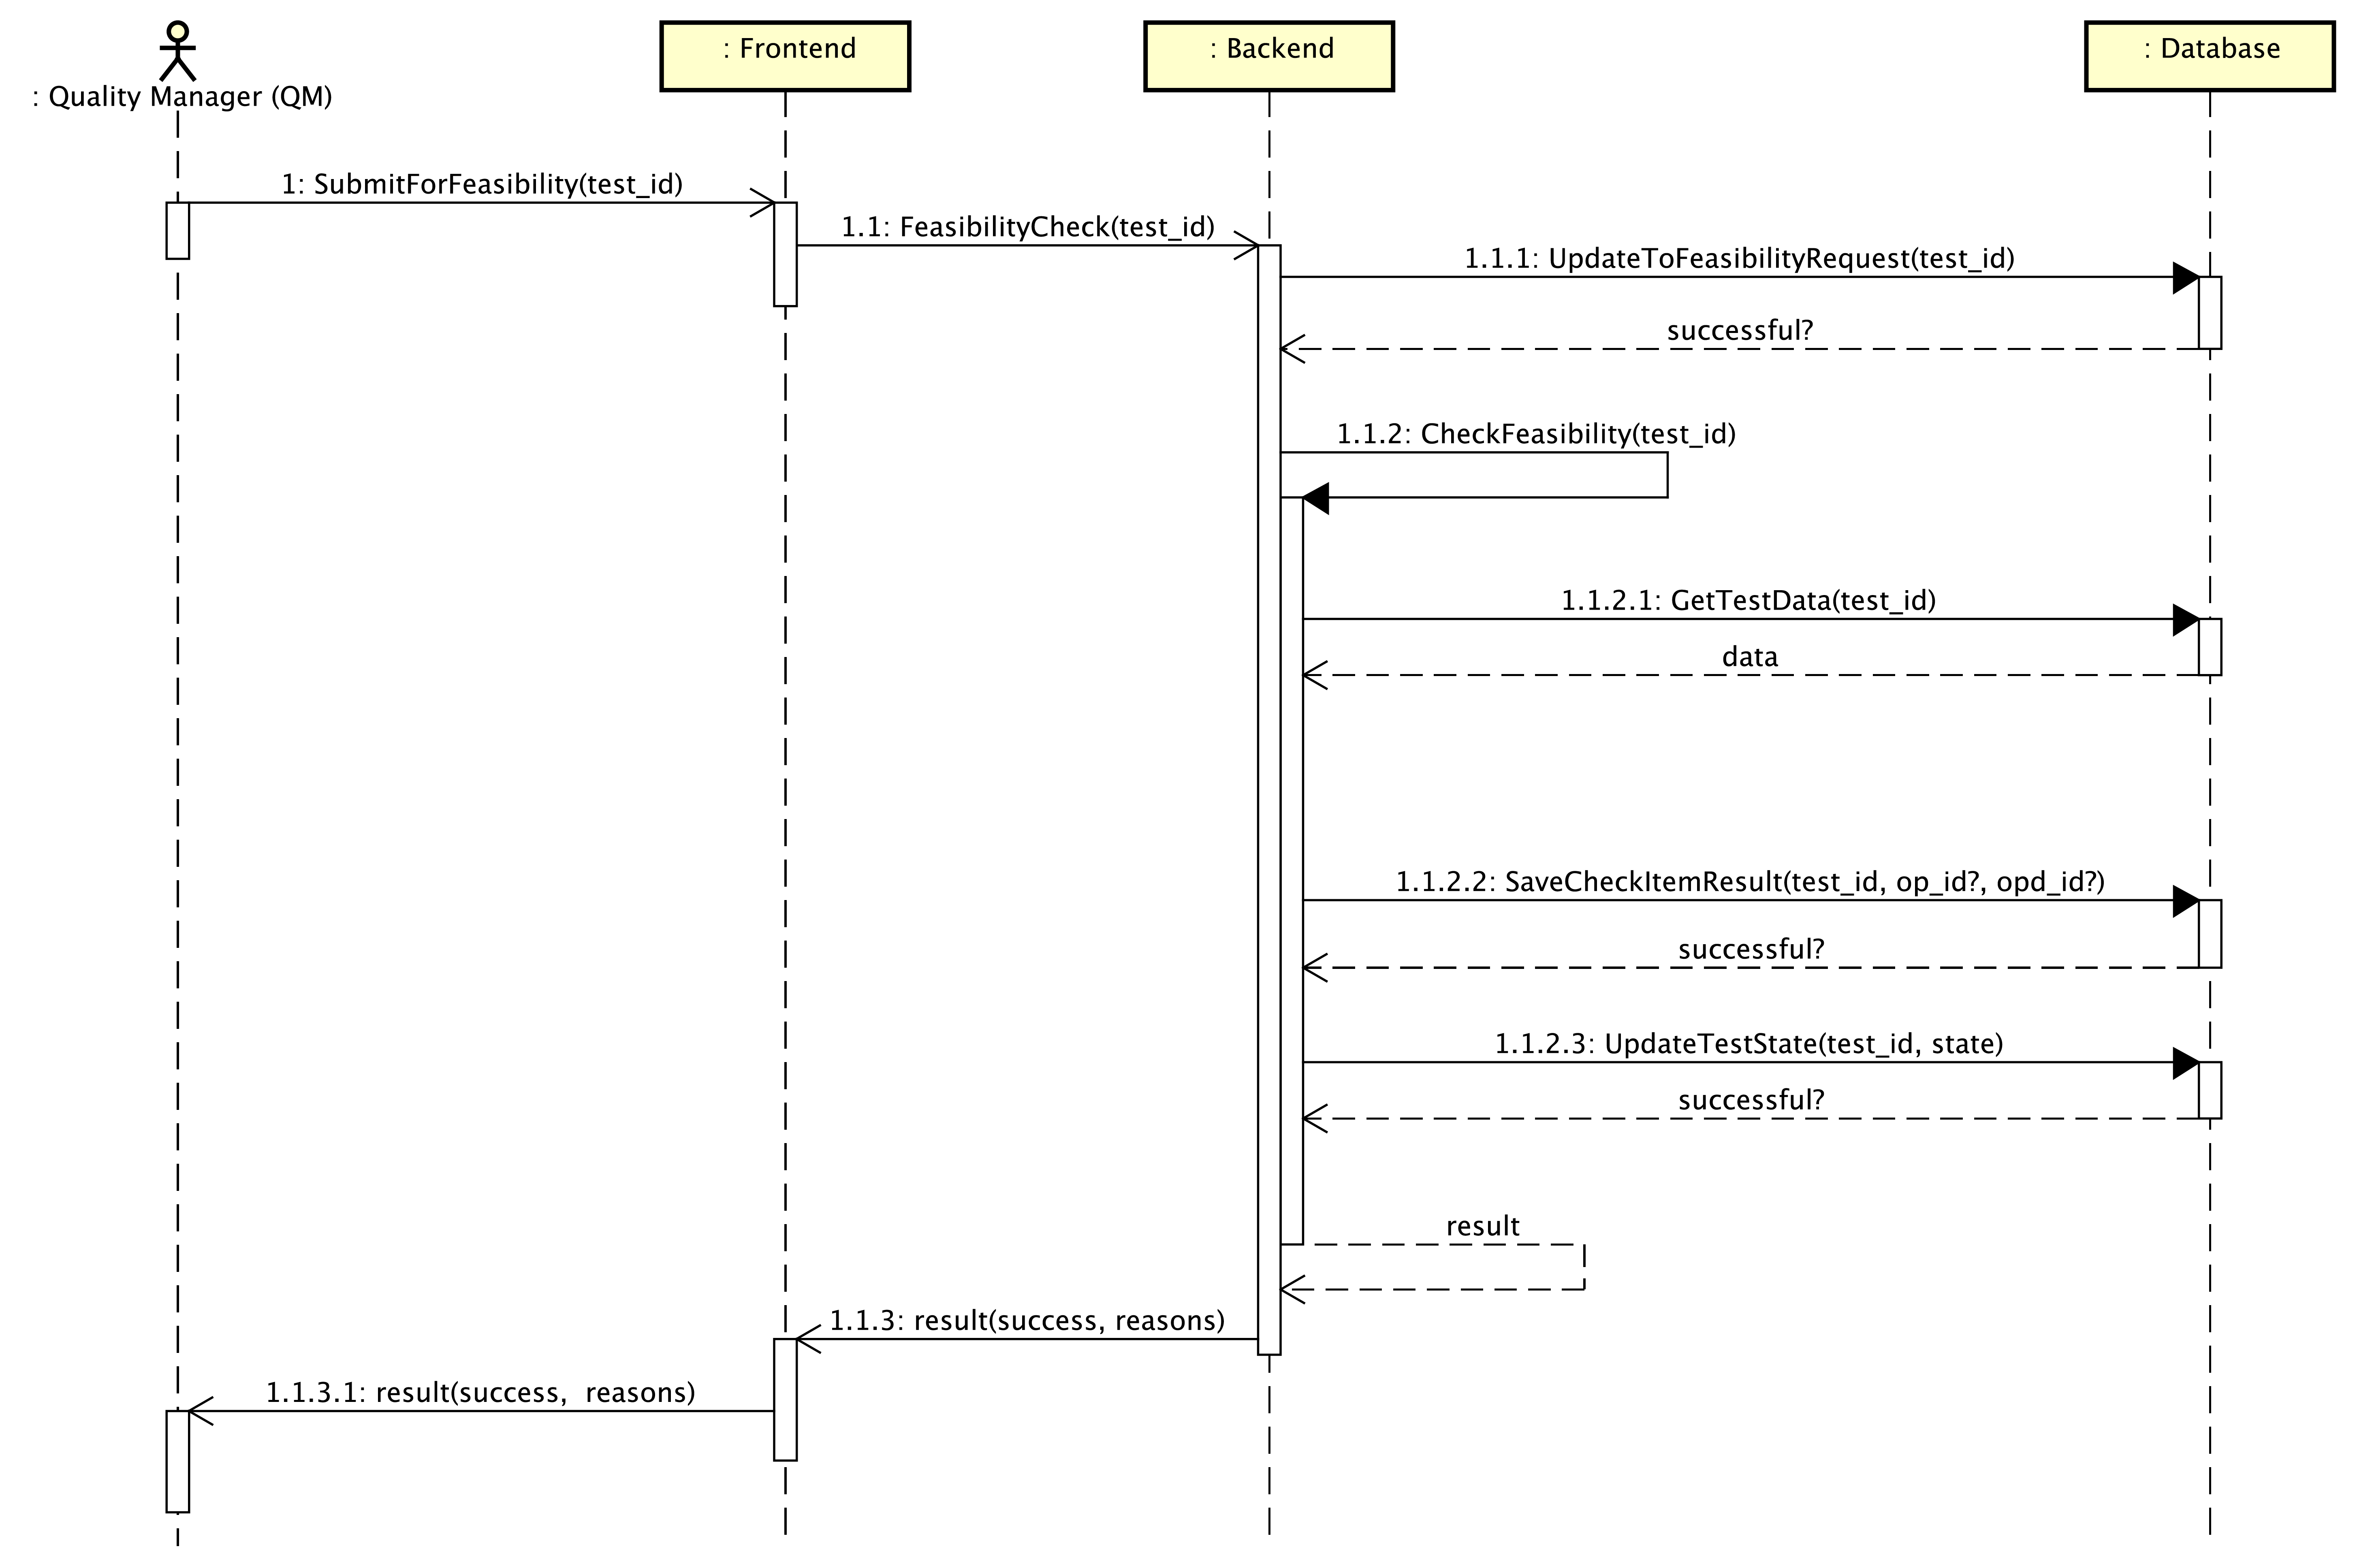
\includegraphics[width=1\textwidth]{bilder/Sequence-Integration.png}
    \caption{Sequenz-Diagramm FeasibilityCheck}
    \label{fig:sequence-diagram}
\end{figure}